\documentclass[11pt]{article}
\usepackage{report}

\title{Self-Organized Criticality \\ Sand pile Model}
\author{Jesper Vesterberg (jumziey@gmail.com)}

\date{\today}

\begin{document}
\begin{titlepage}
  \maketitle
  \thispagestyle{fancy}
  \lhead{
    Department of physics\\
    Umeå Universitet
  }
  \rhead{\today}
  \begin{abstract}
		This report looks at self-organized criticality through the sand pile model. We look our model with walls which make sand disappear if sand crosses it, see its weakness and how to deal with it. We also look closer at how the size of the systems matters for the sizes and the times for the avalanches.
  \end{abstract}
  \cfoot{
		Course: Monte Carlo Methods\\
		Supervisor: Peter Olsson
  }
\end{titlepage}

\lhead{\theauthor}
\rhead{\thetitle\\\today}
\cfoot{\thepage}

\section{Introduction}
We will look at the sand pile model. In this model we have a grid of possible positions for grains of sand. We then add a grain of sand to a random position in the grid. We do this until a grid position has four grains of sand. If this happens an "avalanche" start. The process of "avalanching" is that we move these four grains from the current grid position to all its closest neighbours. If any of its neighbours get four grains in this process the avalanche continue from these neighbouring points. 

We define the size of the avalanche as how many of these grid position gets affected from one avalanche until it stops so we have to start adding grains to get any more effects. The time of an avalanche is defined as how many times we have to continue at neighbouring points. 

In our experiments we first add grains until we have an occupation rate of 52\% in the grid, this so we can remove outliers that will happen during these early update steps. Also if there is a wall instead of a neighbouring grid point we remove this grain of sand and see it as  a "lost grain". 

We will look at how well both size distributions fits into the power law.

\newpage
\section{Avalanche size and time distributions}
Having taken into account the "startup phase" by requiring a certain occupation level in the grid we think we should get pretty good results. Since its the power law ($H(s) \propto s^{-c}$) that should decide how the distribution of avalanches sizes are, we're quite confident that the different system sizes should have a very similar and straight loglog plot. To get a clean result we define bins of a numeric size of 100. If a avalanche occurs within this "binrange" the bin is increased by one. After running our simulation at the length scales of $32,64,128$ and $256$ we got the result depicted in figure~\ref{fig:valueanalysis}.
\begin{figure}[H]
        \centering
        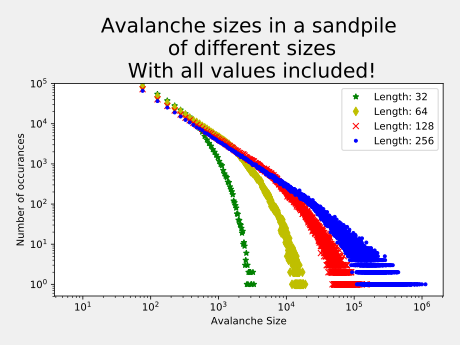
\includegraphics[width=0.9\textwidth]{valueanalysis}
        \caption{Naive loglog plot of the number of occurrences of different sized avalanches when we  dropped one million grains into our grid, started from an occupation level of 52\%, at different length scales. Note the dip, and clear deviation from the expected straight line.}
        \label{fig:valueanalysis}
\end{figure}
But this is not a straight line! What is going on? Well the issue lies in our boundaries. Since we can have avalanches that move out to the walls and then get "quenched" there, it creates a skew. We can see it differs for different length scales on the  simulation too. But if we think of it, the bigger the avalanche, the bigger the chance it is that these hits the wall. Thus for large avalanches we get a smaller chance for them happening since they have to move closer to the middle of the grid for them to not get quenched. And so we get a dip in the number off occurrences for larger avalanches. This we can clearly see in figure~\ref{fig:valueanalysis}. This dip is as expected at larger avalanche sizes for a larger  system. We also note that the smaller systems seem to have a higher occurrences of smaller avalanches, this is also expected since the quenching results in an avalanche to simply become smaller. This effect is spread out more though and manifest like an added constant for all sizes.


By removing these dips we get a picture as seen in figure~\ref{fig:sizes}. This look much more like we had expected. The plot is very similar for the time distribution shown in figure~\ref{fig:times}. We still have that slightly higher occurrences of smaller avalanches for smaller systems due to the effect previously discussed. 
\begin{figure}[H]
        \centering
        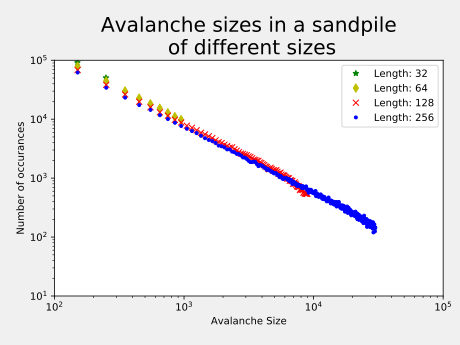
\includegraphics[width=0.9\textwidth]{sizes}
        \caption{A better loglog plot of the number of occurrences of certain avalanche sizes in system with different length scales. Here we removed the dipped caused by the walls in the grid system.}
        \label{fig:sizes}
\end{figure}
\begin{figure}[H]
        \centering
        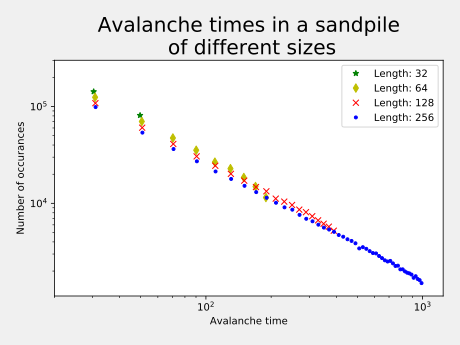
\includegraphics[width=0.9\textwidth]{times}
        \caption{The time distribution of the avalanches are early similar to the size distribution.}
        \label{fig:times}
\end{figure}

\section{Fitting to the power law!}
By assuming that the power law (with $h(s)$ being the occurrence of an avalanche)
\begin{equation}
	H(s) \propto s^{-c}
\end{equation}
hold we can try and figure out this c from using the logarithm on our results. Taking the logarithm yeilds
\begin{equation}
	\log{(H(s))} = -c\log{(s)}
\end{equation}
And since we had an almost constant offset in our loglog plots we assume we have an extra constant
\begin{equation}
	\log{(H(s))} = \log{(k)} -c\log{(s)}
\end{equation}
Under which the power law still holds since this becomes
\begin{equation}
	H(s) = ks^{-c}
\end{equation}
and this still means that $H(s) \propto s^{-c}$.

Doing this fitting yeilds to us a result of $c\approx -1.11$. We have done this fit on the data for the larger length scale since these points are the least effected by an increase of occurrences of small avalanches. This fitted line is depicted in figure~\ref{fig:sizefit}.
\begin{figure}[H]
        \centering
        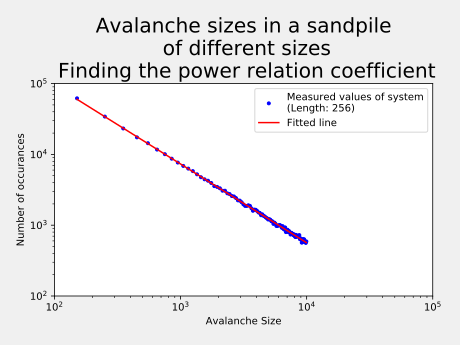
\includegraphics[width=0.9\textwidth]{sizefit}
        \caption{Here we fitted a line to the log:ed data. We can clearly see a nice correlation for a value of $c\approx -1.11$.}
        \label{fig:sizefit}
\end{figure}

\end{document}

